\chapter{Esperimenti e risultati}

Nella fase di sperimentazione del componente ci siamo posti come obiettivo quello di mettere a confronto la simulazione di un modello monolitico e completo con le simulazioni localizzate su specifiche sezioni in cui quest'ultimo è stato diviso. In particolare abbiamo deciso di confrontare il modello completo con due scenari diversi in cui quest'ultimo è stato diviso in 6 e 12 macro regioni adiacenti.

La mappa usata per gli esperimenti è tratta da un blocco residenziale della città di Firenze, in cui abbiamo cercato di inserire topologie diverse, in modo da rappresentare zone come il centro storico, con strade brevi e strette, e i quartieri delle metropoli moderne, con strade di dimensioni maggiori.

La medesima mappa è stata usata dal gruppo di ricerca del Software Science and Technology Laboratory in \cite{esperimenti-sandro} durante la fase di sperimentazione, in cui, inoltre, si è reso utile il componente sviluppato in questo progetto.

\section{Modello monolitico}
La struttura del modello monolitico è rappresentata in Figura \ref{fig:immagine-mappa-completo}. Lo stato iniziale del sistema è di 10000 agenti distribuiti uniformemente in tutto lo spazio disponibile. Quindi le regioni con maggiore densità di strade saranno popolate anche da un numero maggiore di attori. 

\begin{figure}[htbp]
\centering
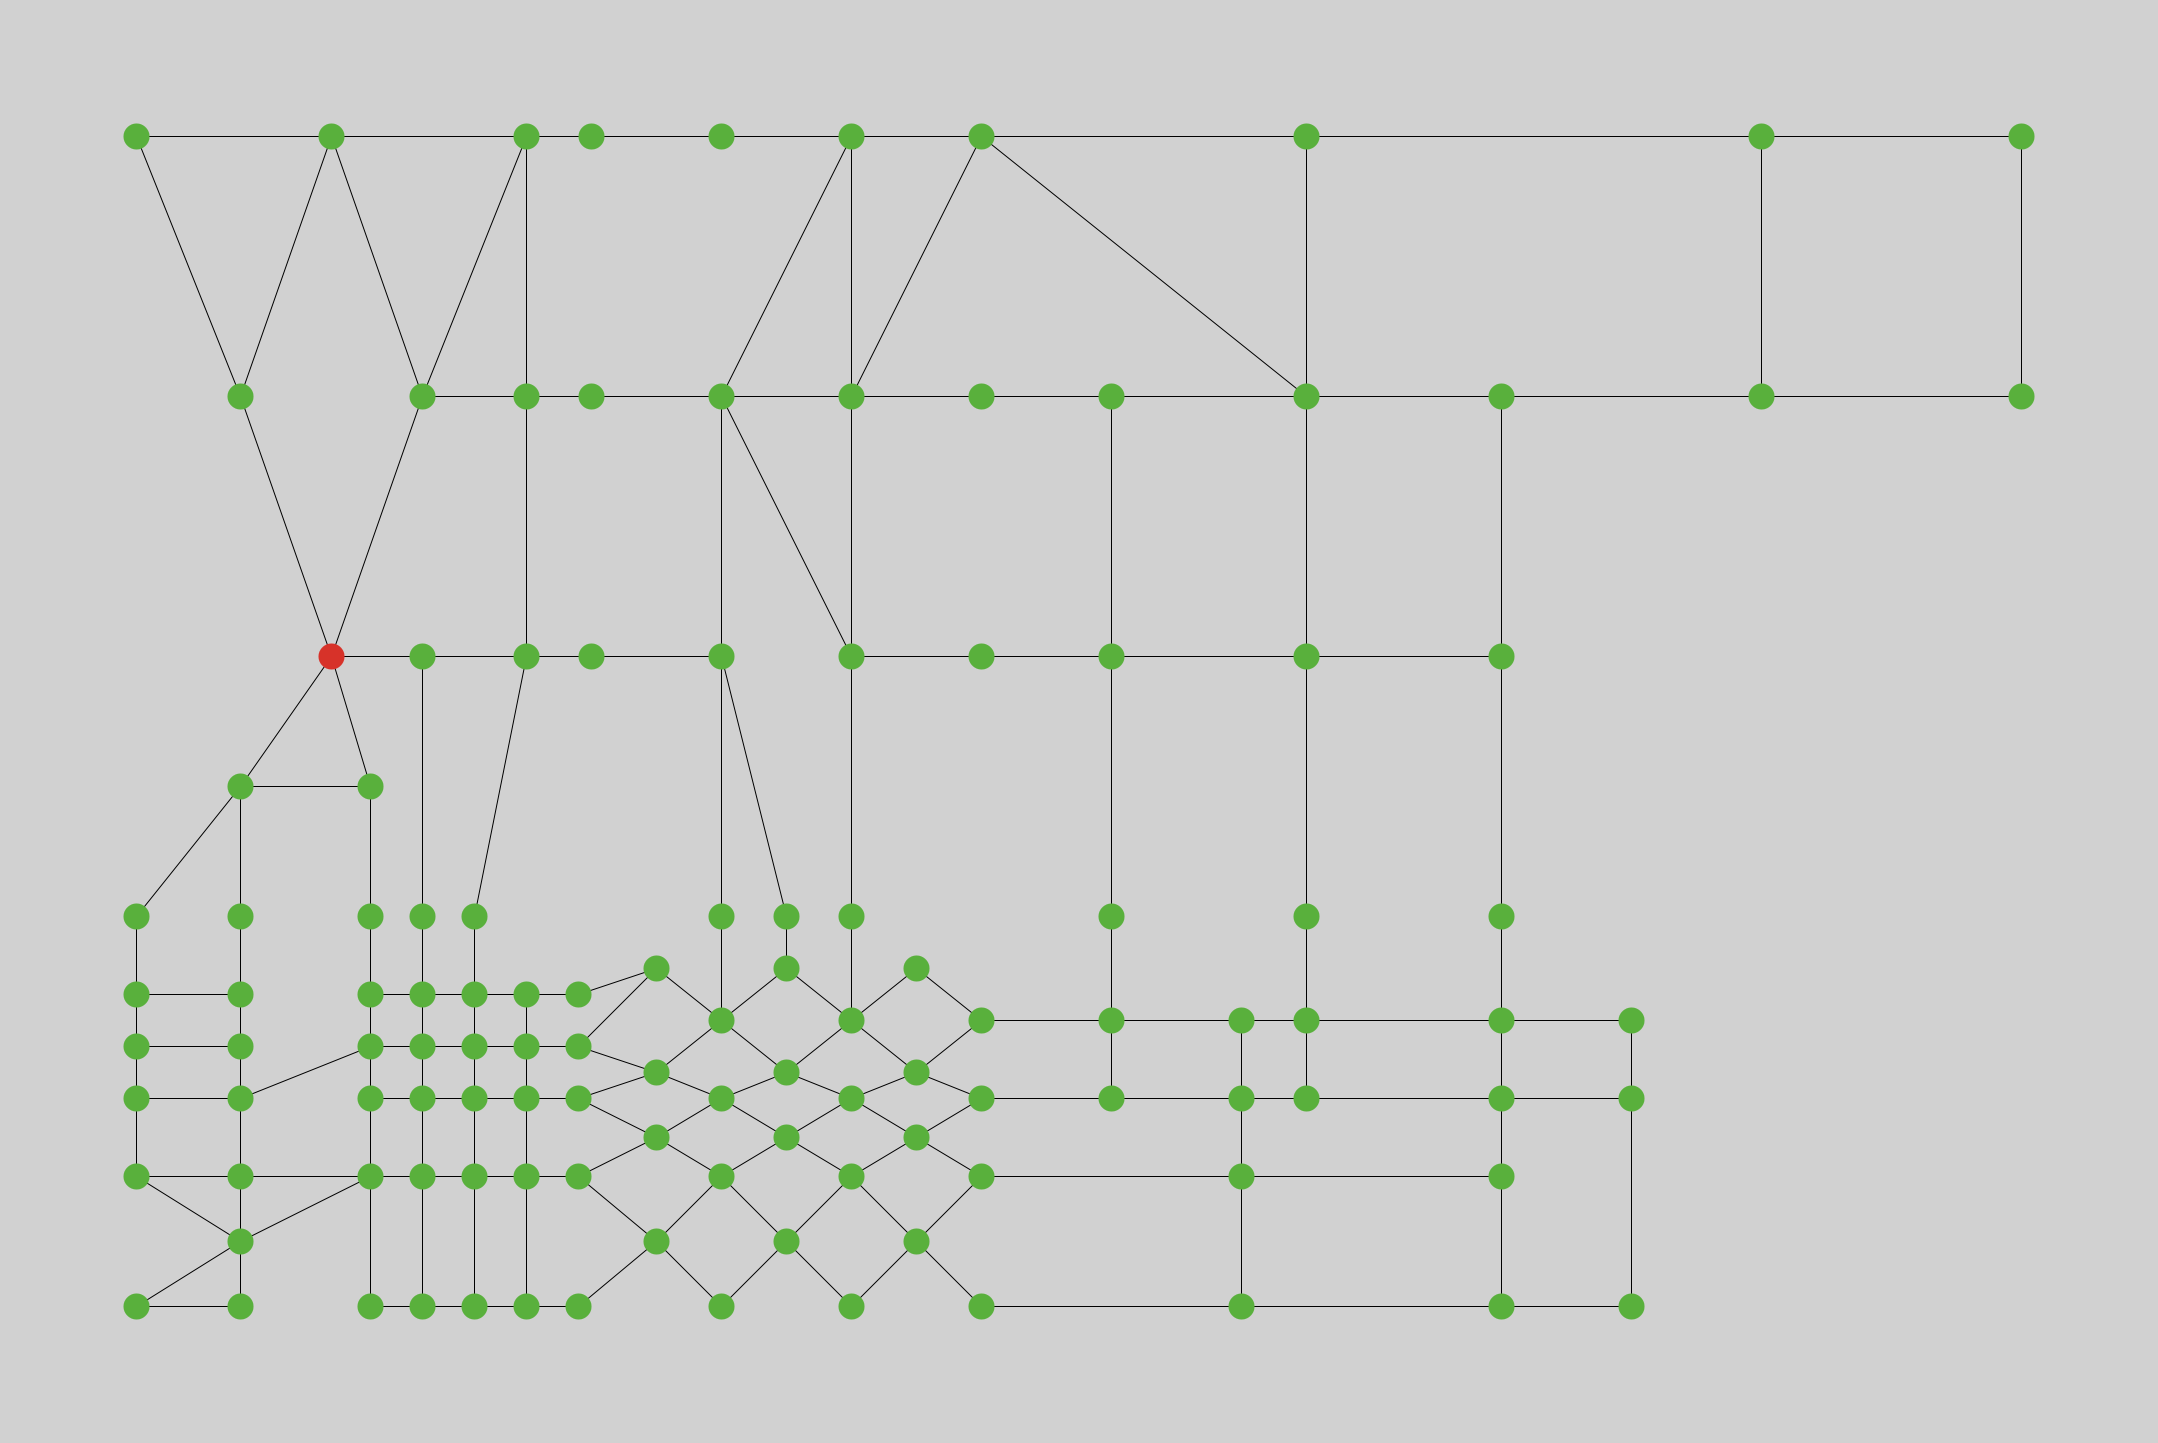
\includegraphics[width=\textwidth,height=\textheight,keepaspectratio]{images/mappa-completo.png}
\caption{Mappa del modello monolitico}
\label{fig:immagine-mappa-completo}
\end{figure}

Per avere una stima sufficientemente rappresentativa del tempo di evacuazione di un ambiente è solitamente necessario eseguire almeno 10 simulazioni dello stesso modello. Nel nostro caso il tempo medio ad eseguire una singola simulazione è 55:58 minuti, quindi per ottenere la stima desiderata sono necessarie circa 9:19:40 ore di simulazioni.

\begin{figure}[htbp]
\centering
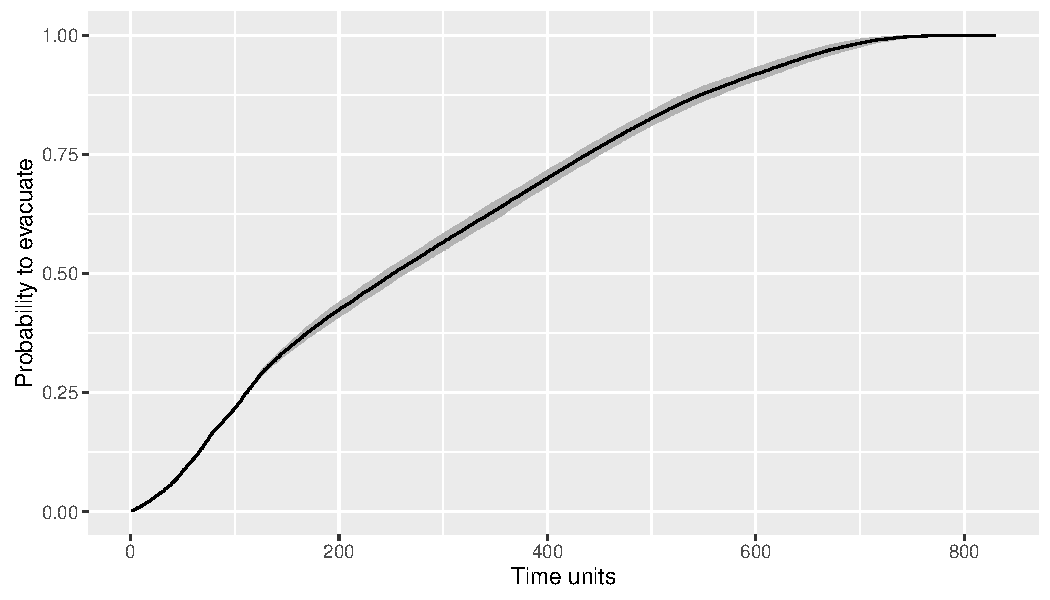
\includegraphics[width=\textwidth,height=\textheight,keepaspectratio]{images/meancdf.pdf}
\caption{Media delle funzioni di distribuzione empiriche della probabilità di aver raggiunto l'uscita al tempo t nel modello monolitico}
\label{fig:ecdf}
\end{figure}

Il gruppo di ricerca del STLAB in \cite{esperimenti-sandro} ha usato le simulazioni eseguite su questo modello come riferimento realistico con cui confrontare le approssimazioni generate a partire dai diversi scenari introdotti. Sono state eseguite 8 simulazioni del medesimo modello in modo da avere una buona approssimazione del tempo medio di evacuazione. Attraverso i dati raccolti i ricercatori hanno generato il grafico in Figura \ref{fig:ecdf} in cui si mostra la ECDF della probabilità di aver evacuato l'ambiente al tempo t.

\section{Scenari con macro regioni}

\begin{figure}[htbp]
\centering
\includegraphics[width=\textwidth,height=\textheight,keepaspectratio]{images/mappa-scenario-A.png}
\includegraphics[width=\textwidth,height=\textheight,keepaspectratio]{images/mappa-scenario-D.png}
\caption{Mappe dei due scenari}
\label{fig:immagine-mappa-completo}
\end{figure}


Nei due scenari A e D la mappa è suddivisa rispettivamente in 6 e 12 sezioni indipendenti in cui i punti di uscita sono punti di connessione con le regioni confinanti. Per ognuna di queste zone sono eseguite simulazioni con 3 diversi stati iniziali, ovvero con densità di affollamento alta, media e bassa. 

Abbiamo inoltre lanciato le simulazioni in due modalità diverse: con densità degli attori costante e transitoria. La modalità con densità costante consiste nel mantenere fisso il numero degli attori all'interno della regione generando un nuovo agente ogni volta che qualcuno raggiunge l'uscita ed eseguendo il modello per un numero prefissato di unità temporali. In questo modo si ottengono informazioni sui tempi di transizione del sistema che si trova in uno stato stabile di affollamento. La modalità transitoria, invece, è la più semplice e rapida delle due, infatti non prevede la generazione di alcun attore, quindi si registrano solo i dati relativi agli agenti che costituiscono lo stato iniziale della regione.

In \cite{esperimenti-sandro} i tempi di transizione ottenuti dai modelli con densità degli attori costante sono usati per calcolare le probabilità di transizione della Catena di Markov che astrae il comportamento dell'attore attraverso le varie regioni come spiegato nella Sezione \ref{sec:approccio-gerarchico}.



\section{Risultati}

Dagli esperimenti condotti abbiamo misurato i tempi necessari ad eseguire un numero consistente di simulazioni dalle quali estrarre i tempi di transizione dei vari attori. Nella Tabella \ref{tab:tabella-confronto} sono confrontati il modello monolitico e i due scenari sia con approccio a densità costante che transitorio. 

\begin{table}[h]
  \centering
  \resizebox{0.7\textwidth}{!} {
  \begin{tabular}{ |l|l|l| }
	\hline
	\textbf{Scenario}	&		\textbf{densità costante}	&		\textbf{transitorio}	\\ \hline
	\textbf{Monolitico} &		 						&		9:19:40		\\ \hline
	\textbf{A}			 &		21:33:36 				&		0:21:51		\\ \hline
	\textbf{D}			 &		4:49:27 				&		0:23:13		\\ \hline

  \end{tabular}
  }
  \caption{Confronto dei tempi complessivi di simulazione}
  \label{tab:tabella-confronto}
\end{table}

La prima cosa da osservare è che il tempo totale di simulazione del modello completo è minore di quello necessario ad eseguire tutte le simulazioni sulle varie regioni dello scenario A con metodo a densità costante. Nello scenario D invece il tempo totale delle simulazioni con il medesimo metodo è comunque minore di quello di riferimento del modello monolitico. Il vantaggio che questo approccio porta, però, si manifesta nel momento in cui si vogliono studiare le conseguenze di piccole modifiche apportate in certe regioni. Infatti nel caso del modello monolitico si devono eseguire nuovamente le simulazioni su tutto l'ambiente, mentre nei due scenari si possono eseguire simulazioni isolate alla specifica regione, riducendo drasticamente il tempo necessario per la misura dei nuovi dati. Ad esempio se volessimo valutare i tempi di evacuazione del modello eliminando alcune strade della zona A2, nel caso del modello monolitico, per ottenere nuovamente tutti i dati sarebbero necessarie sempre circa 9 ore, al contrario nello scenario A potremmo lanciare simulazioni solo per la zona interessata e quindi impiegare solo circa 2 ore per l'ottenimento dei nuovi dati.
 
\begin{table}[h]
  \centering
  \resizebox{0.7\textwidth}{!} {
  \begin{tabular}[t]{ |l|l|l| }
	\hline
	\textbf{Regione}	&		\textbf{Densità costante}	&		\textbf{Transitorio}	\\ \hline
	\textbf{A1} 		&		3:16:25					&		0:03:06			\\ \hline
	\textbf{A2}			 &		2:13:11 				&		0:02:40		\\ \hline
	\textbf{A3}			 &		5:12:48 				&		0:03:40		\\ \hline
	\textbf{A4}			 &		6:20:39 				&		0:06:08			\\ \hline
	\textbf{A5}			 &		2:36:25 				&		0:03:29		\\ \hline
	\textbf{A6}			 &		1:46:20 				&		0:02:46		\\ \hline

  \end{tabular}
  
  }
  \caption{Tempi di simulazione relativi alle singole regioni dello scenario A con metodo a densità costante e transitorio}
  \label{tab:tabella-dati-simulazioni-A}
\end{table}

\begin{table}[h]
  \centering
  \resizebox{0.7\textwidth}{!} {
 \begin{tabular}[t]{ |l|l|l| }
	 	\hline
	\textbf{Regione}	&		\textbf{Densità costante}	&		\textbf{Transitorio}	\\ \hline
	\textbf{D1} 	 &		0:27:26					&		0:01:56		\\ \hline
	\textbf{D2}		 &		0:29:15 				&		0:02:03		\\ \hline
	\textbf{D3}		 &		0:49:46 				&		0:01:58		\\ \hline
	\textbf{D4}		 &		0:29:48 				&		0:02:00		\\ \hline
	\textbf{D5}		 &		0:42:43 				&		0:01:51		\\ \hline
	\textbf{D6}		 &		0:37:23 				&		0:01:40		\\ \hline
	\textbf{D7}		 &		0:12:58 				&		0:01:58		\\ \hline
	\textbf{D8}		 &		0:11:20 				&		0:02:07		\\ \hline
	\textbf{D9}		 &		0:23:57 				&		0:01:58		\\ \hline
	\textbf{D10}	 &		0:21:52 				&		0:02:06		\\ \hline
	\textbf{D11}	 &		0:02:08 				&		0:01:43		\\ \hline
	\textbf{D12}	 &		0:0:52 					&		0:01:48		\\ \hline
	
	
  \end{tabular}
  
  }
  \caption{Tempi di simulazione relativi alle singole regioni dello scenario D con metodo a densità costante e transitorio}
  \label{tab:tabella-dati-simulazioni-D}
\end{table}
 
La natura modulare del modello nei due scenari, quindi, ci permette uno studio dei movimenti delle masse molto più flessibile, riducendo considerevolmente il costo del calcolo della soluzione rispetto al modello monolitico.

I ricercatori del STLAB nel loro lavoro di sperimentazione in \cite{esperimenti-sandro} hanno generato il grafico in Figura \ref{fig:scenariosAD} in cui è mostrato il confronto tra la probabilità di aver raggiunto l'uscita al tempo t del modello monolitico e l'approssimazione ottenuta dai due scenari usando la tecnica del campo medio.

\begin{figure}[htbp]
\centering
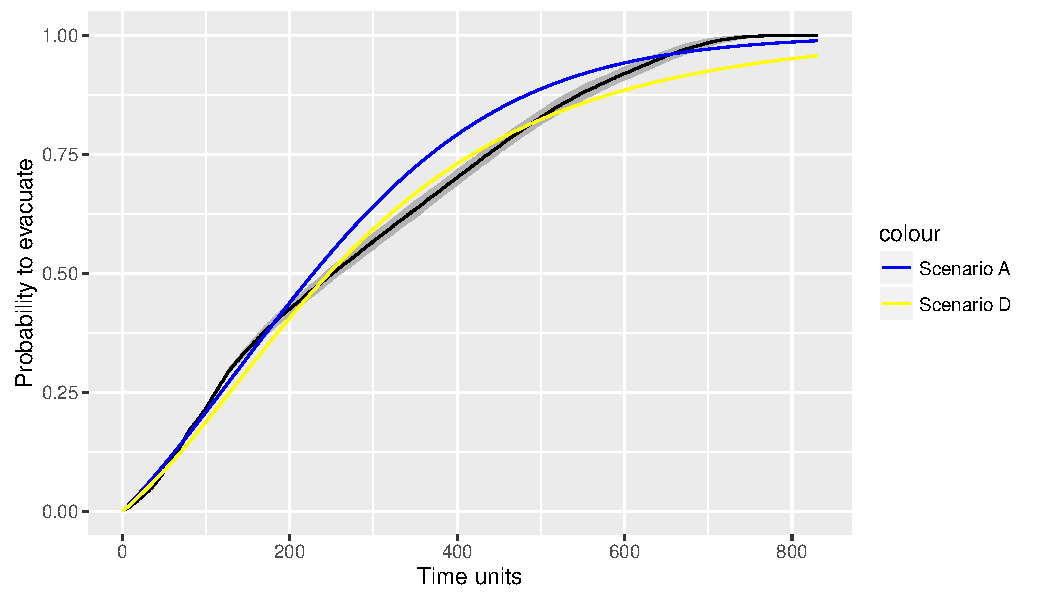
\includegraphics[width=.8\textwidth,height=\textheight,keepaspectratio]{images/scenariosAD.pdf}
\caption{Probabilità di aver raggiunto l'uscita al tempo t per i due scenari}
\label{fig:scenariosAD}
\end{figure}

Inoltre in Figura \ref{fig:errorsplotAD} è mostrato l'errore commesso dalle approssimazioni rispetto al sistema completo. Da questi risultati si osserva che le approssimazioni introdotte hanno un comportamento simile al modello monolitico, con una accuratezza diversa al variare degli scenari.

\begin{figure}[htbp]
\centering
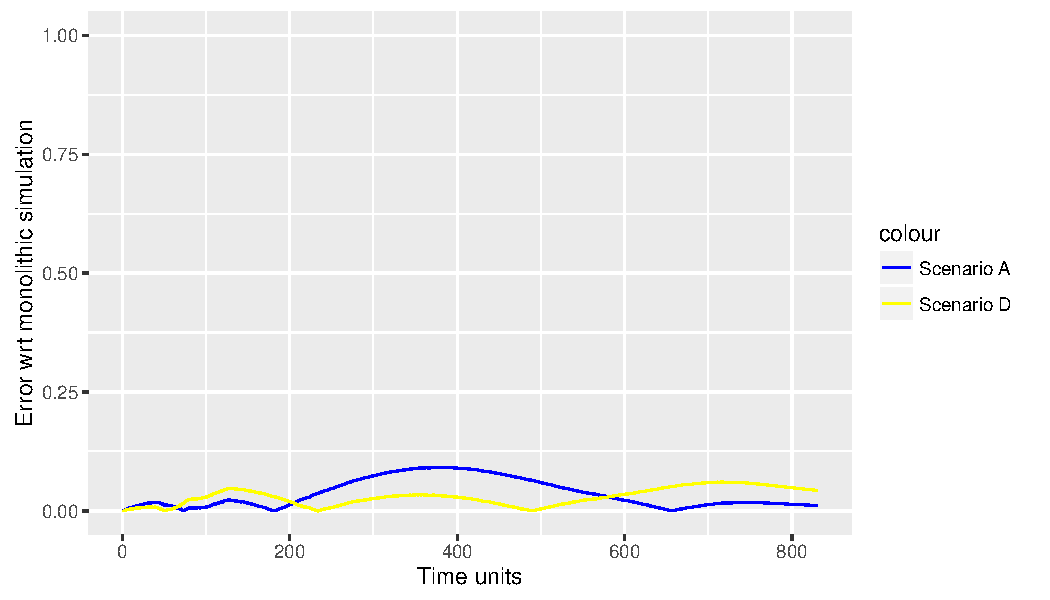
\includegraphics[width=.8\textwidth,height=\textheight,keepaspectratio]{images/errorplotAD.pdf}
\caption{Errore delle approssimazioni introdotte dagli scenari rispetto al modello monolitico}
\label{fig:errorsplotAD}
\end{figure}



 